\documentclass[14pt]{extbook}
\usepackage{multicol, enumerate, enumitem, hyperref, color, soul, setspace, parskip, fancyhdr} %General Packages
\usepackage{amssymb, amsthm, amsmath, latexsym, units, mathtools} %Math Packages
\everymath{\displaystyle} %All math in Display Style
% Packages with additional options
\usepackage[headsep=0.5cm,headheight=12pt, left=1 in,right= 1 in,top= 1 in,bottom= 1 in]{geometry}
\usepackage[usenames,dvipsnames]{xcolor}
\usepackage{dashrule}  % Package to use the command below to create lines between items
\newcommand{\litem}[1]{\item#1\hspace*{-1cm}\rule{\textwidth}{0.4pt}}
\pagestyle{fancy}
\lhead{Progress Quiz 9}
\chead{}
\rhead{Version A}
\lfoot{9541-5764}
\cfoot{}
\rfoot{Summer C 2021}
\begin{document}

\begin{enumerate}
\litem{
Solve the rational equation below. Then, choose the interval(s) that the solution(s) belongs to.\[ \frac{-30}{35x -10} + 1 = \frac{-30}{35x -10} \]\begin{enumerate}[label=\Alph*.]
\item \( x \in [0.29,2.29] \)
\item \( \text{All solutions lead to invalid or complex values in the equation.} \)
\item \( x \in [-0.4,0.2] \)
\item \( x_1 \in [-0.4, 0.2] \text{ and } x_2 \in [-0.71,2.29] \)
\item \( x_1 \in [0.2, 0.8] \text{ and } x_2 \in [-0.71,2.29] \)

\end{enumerate} }
\litem{
Choose the graph of the equation below.\[ f(x) = \frac{1}{(x - 2)^2} - 2 \]\begin{enumerate}[label=\Alph*.]
\begin{multicols}{2}\item 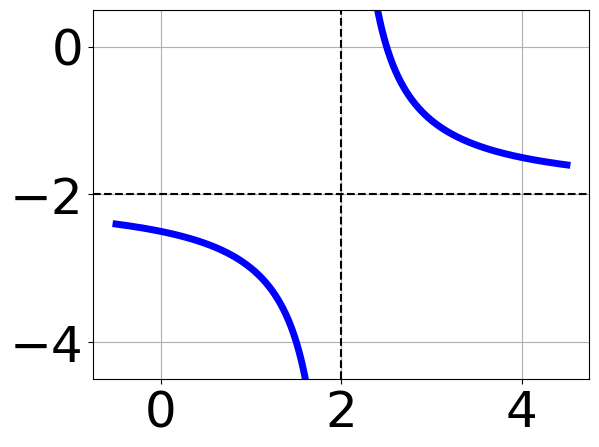
\includegraphics[width = 0.3\textwidth]{../Figures/rationalEquationToGraphCopyAA.png}\item 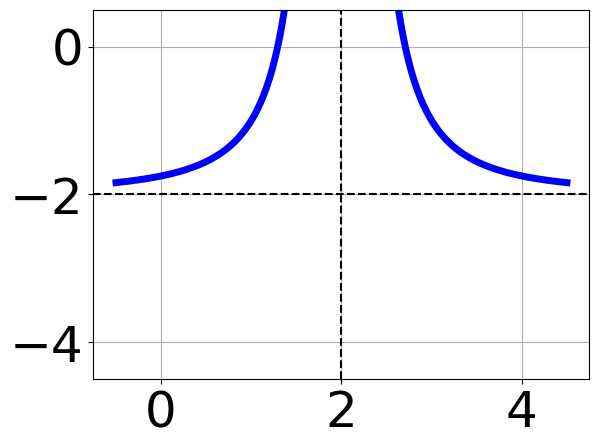
\includegraphics[width = 0.3\textwidth]{../Figures/rationalEquationToGraphCopyBA.png}\item 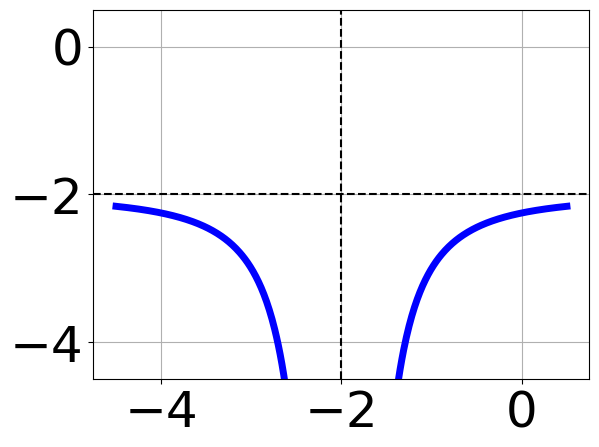
\includegraphics[width = 0.3\textwidth]{../Figures/rationalEquationToGraphCopyCA.png}\item 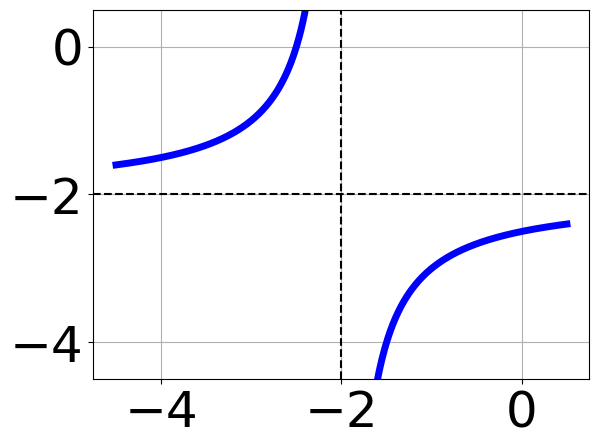
\includegraphics[width = 0.3\textwidth]{../Figures/rationalEquationToGraphCopyDA.png}\end{multicols}\item None of the above.
\end{enumerate} }
\litem{
Solve the rational equation below. Then, choose the interval(s) that the solution(s) belongs to.\[ \frac{2x}{7x + 2} + \frac{-5x^{2}}{-35x^{2} -31 x -6} = \frac{4}{-5x -3} \]\begin{enumerate}[label=\Alph*.]
\item \( x \in [-0.53,0.55] \)
\item \( \text{All solutions lead to invalid or complex values in the equation.} \)
\item \( x_1 \in [-2.69, -1.04] \text{ and } x_2 \in [-0.27,-0.24] \)
\item \( x \in [-0.88,-0.31] \)
\item \( x_1 \in [-2.69, -1.04] \text{ and } x_2 \in [-0.3,-0.28] \)

\end{enumerate} }
\litem{
Determine the domain of the function below.\[ f(x) = \frac{6}{36x^{2} +54 x + 20} \]\begin{enumerate}[label=\Alph*.]
\item \( \text{All Real numbers except } x = a, \text{ where } a \in [-30.08, -29.84] \)
\item \( \text{All Real numbers.} \)
\item \( \text{All Real numbers except } x = a \text{ and } x = b, \text{ where } a \in [-0.86, -0.73] \text{ and } b \in [-0.73, -0.5] \)
\item \( \text{All Real numbers except } x = a, \text{ where } a \in [-0.86, -0.73] \)
\item \( \text{All Real numbers except } x = a \text{ and } x = b, \text{ where } a \in [-30.08, -29.84] \text{ and } b \in [-24.13, -23.8] \)

\end{enumerate} }
\litem{
Solve the rational equation below. Then, choose the interval(s) that the solution(s) belongs to.\[ \frac{-9}{4x -4} + -6 = \frac{-6}{-20x + 20} \]\begin{enumerate}[label=\Alph*.]
\item \( x_1 \in [-3.42, 0.57] \text{ and } x_2 \in [0.49,0.7] \)
\item \( x \in [-3.42,0.57] \)
\item \( x_1 \in [0.57, 3.58] \text{ and } x_2 \in [0.74,1.39] \)
\item \( \text{All solutions lead to invalid or complex values in the equation.} \)
\item \( x \in [0.57,1.57] \)

\end{enumerate} }
\litem{
Choose the equation of the function graphed below.
\begin{center}
    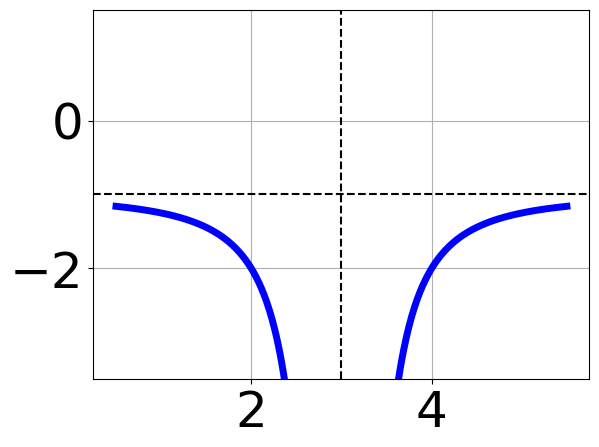
\includegraphics[width=0.5\textwidth]{../Figures/rationalGraphToEquationA.png}
\end{center}
\begin{enumerate}[label=\Alph*.]
\item \( f(x) = \frac{-1}{(x - 3)^2} - 1 \)
\item \( f(x) = \frac{1}{(x + 3)^2} - 1 \)
\item \( f(x) = \frac{1}{x + 3} - 1 \)
\item \( f(x) = \frac{-1}{x - 3} - 1 \)
\item \( \text{None of the above} \)

\end{enumerate} }
\litem{
Solve the rational equation below. Then, choose the interval(s) that the solution(s) belongs to.\[ \frac{-3x}{-6x -7} + \frac{-6x^{2}}{-30x^{2} -47 x -14} = \frac{-3}{5x + 2} \]\begin{enumerate}[label=\Alph*.]
\item \( x_1 \in [-1.64, -0.93] \text{ and } x_2 \in [-0.7,1.1] \)
\item \( x \in [-1.64,-0.93] \)
\item \( x \in [-0.54,-0.38] \)
\item \( \text{All solutions lead to invalid or complex values in the equation.} \)
\item \( x_1 \in [-0.6, -0.44] \text{ and } x_2 \in [-3.7,-1.3] \)

\end{enumerate} }
\litem{
Choose the graph of the equation below.\[ f(x) = \frac{-1}{(x - 3)^2} - 2 \]\begin{enumerate}[label=\Alph*.]
\begin{multicols}{2}\item 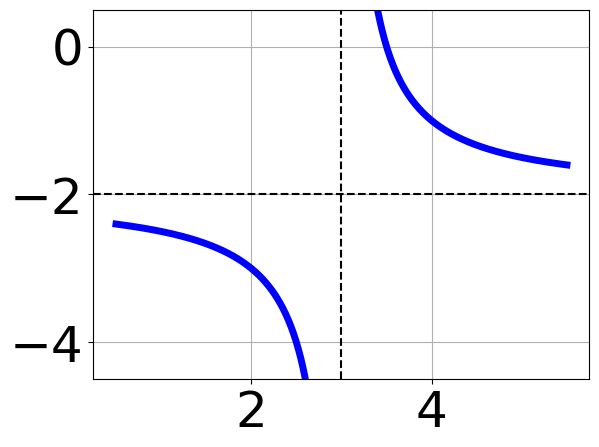
\includegraphics[width = 0.3\textwidth]{../Figures/rationalEquationToGraphAA.png}\item 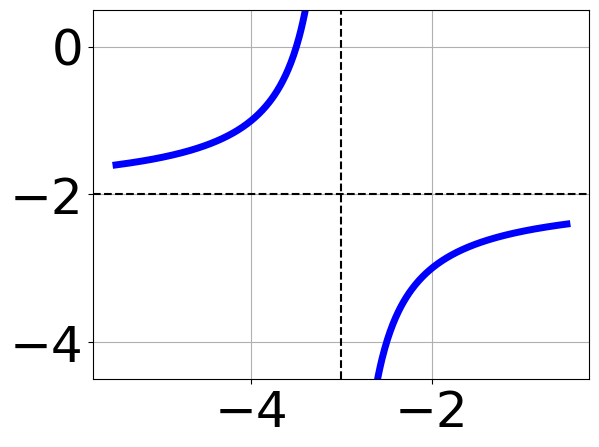
\includegraphics[width = 0.3\textwidth]{../Figures/rationalEquationToGraphBA.png}\item 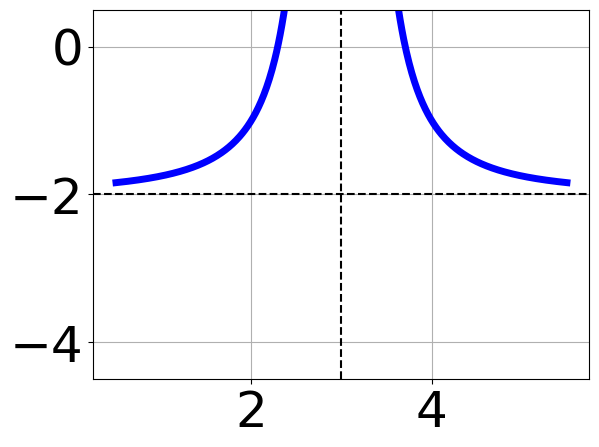
\includegraphics[width = 0.3\textwidth]{../Figures/rationalEquationToGraphCA.png}\item 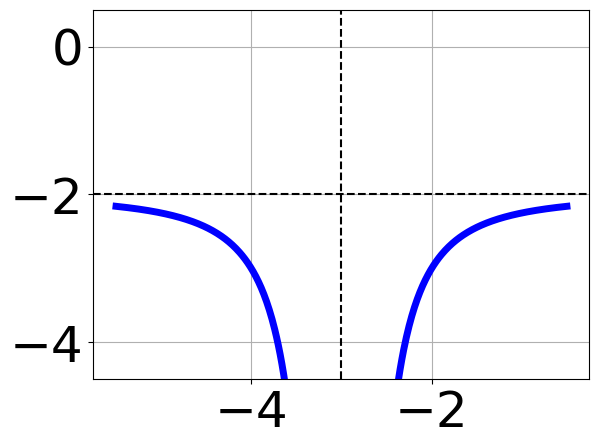
\includegraphics[width = 0.3\textwidth]{../Figures/rationalEquationToGraphDA.png}\end{multicols}\item None of the above.
\end{enumerate} }
\litem{
Choose the equation of the function graphed below.
\begin{center}
    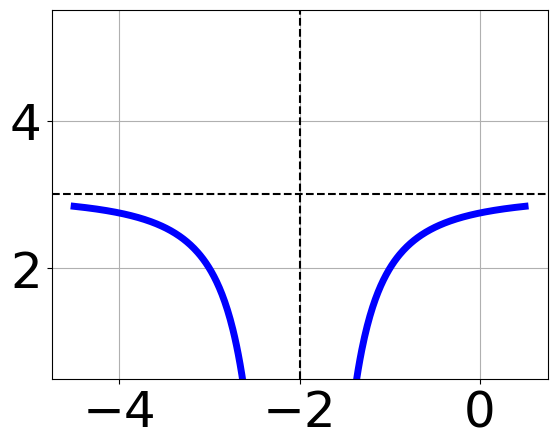
\includegraphics[width=0.5\textwidth]{../Figures/rationalGraphToEquationCopyA.png}
\end{center}
\begin{enumerate}[label=\Alph*.]
\item \( f(x) = \frac{-1}{(x + 2)^2} + 3 \)
\item \( f(x) = \frac{1}{x - 2} + 3 \)
\item \( f(x) = \frac{1}{(x - 2)^2} + 3 \)
\item \( f(x) = \frac{-1}{x + 2} + 3 \)
\item \( \text{None of the above} \)

\end{enumerate} }
\litem{
Determine the domain of the function below.\[ f(x) = \frac{5}{15x^{2} +42 x + 24} \]\begin{enumerate}[label=\Alph*.]
\item \( \text{All Real numbers except } x = a \text{ and } x = b, \text{ where } a \in [-20.36, -19.15] \text{ and } b \in [-18.44, -17.43] \)
\item \( \text{All Real numbers except } x = a, \text{ where } a \in [-2.3, -1.32] \)
\item \( \text{All Real numbers.} \)
\item \( \text{All Real numbers except } x = a, \text{ where } a \in [-20.36, -19.15] \)
\item \( \text{All Real numbers except } x = a \text{ and } x = b, \text{ where } a \in [-2.3, -1.32] \text{ and } b \in [-1, -0.34] \)

\end{enumerate} }
\end{enumerate}

\end{document}